%&pdflatex
\documentclass[12pt]{article}


\usepackage{graphicx}
\graphicspath{ {images/} }
\usepackage{colortbl}
\usepackage{xr}
\usepackage{longtable}
\usepackage{xfrac}
\usepackage{tabularx}
\usepackage{booktabs}
\usepackage{hyperref}
\usepackage{xcolor} % for different colour comments
\usepackage{fullpage}
\newcounter{rowcount}
\setcounter{rowcount}{0}
\usepackage{tikz}
\usetikzlibrary{shapes,arrows}


%% Diagram formatting
\tikzstyle{block} = [draw, rectangle, minimum height=1.5em, minimum
width=2em, text centered]
\tikzstyle{arrow} = [thick,-,>=stealth]


\hypersetup{
    bookmarks=true,         % show bookmarks bar?
    colorlinks=true,        % false: boxed links; true: colored links
    linkcolor=blue,        % color of internal links (change box color with linkbordercolor)
    citecolor=green,        % color of links to bibliography
    filecolor=magenta,      % color of file links
    urlcolor=cyan           % color of external links
}

%% Comments
\newif\ifcomments\commentstrue
\ifcomments
\newcommand{\authornote}[3]{\textcolor{#1}{[#3 ---#2]}}
\newcommand{\todo}[1]{\textcolor{red}{[TODO: #1]}}
\else
\newcommand{\authornote}[3]{}
\newcommand{\todo}[1]{}
\fi
\newcommand{\wss}[1]{\authornote{magenta}{SS}{#1}}
\newcommand{\ds}[1]{\authornote{blue}{DS}{#1}}
\newcommand{\kly}[1]{\authornote{green}{KL}{#1}}
\newcommand{\cc}[1]{\authornote{orange}{CC}{#1}}

%%%%%%%%%%%%%%%%%%%%%%%%%%%%%

\begin{document}

    \title{User Manual}
    \author{Team 6\\ \\James Anthony (anthonjb)\\ Wenqiang Chen (chenw25)\\ Carolyn Chong
        (chongce)\\ Kevin Ly (lyk2)}
    \date{\today}

    \maketitle

    \pagebreak

    \tableofcontents
    \listoffigures

    \section*{Revision History}
    \begin{tabular}{|c|c|}
        \hline
        \textbf{Date}  & \textbf{Comments} \\ \hline
        February 28, 2016 & Revision 0 \\ \hline
    \end{tabular}

    \pagebreak

    %%%%%%%%%%%%%%%%%%%%%%%%%%%%%

    %%%%%%%%%%%%%%%%%%%%%%%%%%%%%% Introduction
    \section{Introduction}

    Words

    %%%%%%%%%%%%%%%%%%%%%%%%%%%%%% Copyright
    \section{Copyright Information}
    The Quarters: The Living Network is owned and managed by Team 6 of CS4ZP6 apart of McMaster University. Collaborators include Kevin Ly, Carolyn Chong, Wenchiang Chen, James Anthony. This is an open source project hosted on GitHub. Fair usage with Common Development an Distribution License (CDDL-1.0).

    %%%%%%%%%%%%%%%%%%%%%%%%%%%%%% About this Manual
    \section{About this Manual}

    %%%%%%%%%%%%%%%%%%%%%%%%%%%%%%
    \section{Browser Requirements}
    Quarters is an online web application, avaliable to all browers with internet connection, HTML5, CSS3, Javascript-enabled. Below are compatiable browers:
    \begin{itemize}
        \item Microsoft Internet Explorer (10 +)
        \item Microsoft Edge (any)
        \item Google Chrome (any)
        \item Mozilla Firefox (13 +)
    \end{itemize}

    %%%%%%%%%%%%%%%%%%%%%%%%%%%%%% Tasks
    \section{Tasks}

    \subsection{Registration}
    \label{sec:registration}
    All user must have a registered account before using Quarters. Registration process is simple and easy, only a valid email and a password is required.\\\\
    You can create an account by following these instructions:

    \begin{enumerate}
        \item Click on "SIGN UP" button on the top of the homepage, or Click on "LOGIN" button then select "Register" tab
        \item Enter a valid email address and password
        \item Click on "REGISTER NOW"
        \item An email will be sent to the specified email address, which will contain a link for you to activate your account.
    \end{enumerate}
    \subsection{Login}
    All user must be logged in to use any of the Quarters' features. If you do you have an account, please refer to \hyperref[sec:registration]{Registration} to create an account. \\ \\
    You can login by following these instructions:
    \begin{enumerate}
        \item Click on "LOGIN" on the top of the homepage, or Click on "SIGN UP" button and switch to "Login" tab
        \item Enter your registered email address and password
        \item Click on "LOG IN"
    \end{enumerate}
    \subsection{House Management} %%%%
    If the user has just registered on Quarters and they are not yet a member of a house, the user shall be prompted with a modal window asking them to either Join or Create a house. If the user is already a member of a house this same modal can be accessed by pressing the House Management button on the  left side of the navigation bar at the top of the page. ****** ADD IMAGE OF THE HOUSE MANAGEMENT BUTTON HERE ******

    \subsubsection{Create House}
    \begin{enumerate}
        \item From the House Management modal window, press the ``Create'' button, which can be found in the bottom right corner of the modal window. The contents of the modal window will now display a form that the user must complete in order to create the house.
        \item Once all of the required fields have been completed (required fields are labeled), press the ``Create'' button, which can be found in the bottom right corner of the modal window. From here the user will be redirected to the House Management modal.
    \end{enumerate}

    \subsubsection{Join House}
    \begin{enumerate}
        \item From the House Management modal window, press the ``Join New'' button, which can be hound in the bottom right corner of the modal window. The contents of the modal window will now display a text field labeled ``Invitation Code''.
        \item Enter the invitation code corresponding to the house they wish to join, and then press the ``Join'' button, which can be found in the bottom right corner of the modal window. From here the user will be redirected to the House Management modal.
    \end{enumerate}

    \subsubsection{Leave House}
    \begin{enumerate}
        \item From the House Management modal window the user shall select the house that they wish to leave by using the radio buttons associated with each house.
        \item Once the house has been selected, press the ``Leave House'' button, which can be found at the top left of the modal window. A new modal window will then pop up, asking the user to confirm that they want to leave the house.
        \item Press the ``OK'' button at the bottom right of the modal window. From here the user will be redirected to the House Management modal, and the house that they left will no longer be included in the list of available houses.
    \end{enumerate}

    \subsubsection{Set Default House}
    \begin{enumerate}
        \item From the House Management modal window the user shall select the house that they wish to set as default by using the radio buttons associated with each house.
        \item Once the house has been selected, press the ``Set Default'' button, which can be found at the top left of the modal window. From here the user will be redirected to the House Management modal, and the house that they set as default will already be selected (indicated by the radio button associated with the house).
    \end{enumerate}

    \subsubsection{Select House}
    \begin{enumerate}
        \item From the House Management modal window the user shall select the house that they wish to select by using the radio buttons associated with each house.
        \item Once the house has been selected, press the ``Select'' button, which can be found at the bottom right of the modal window. From here the user will be redirected to the House Management modal. The contents of the rest of the site will now correspond to the house that the user has selected.
    \end{enumerate}

    \subsection{User Profile} %%%%
    \subsubsection{View User Profile}
    \begin{enumerate}
        \item On the right side of the navigation bar, found at the top of the page, the email address of the user will be displayed with an arrow indicating a drop down menu. Press this button to reveal the ``User profile'' option.
        \item Press the ``User Profile'' option. From here the user will be able to see all of the information relevant to their account.
    \end{enumerate}

    \subsubsection{Edit User Profile Information}
    (Note: Users are only able to edit their own information)
    \begin{enumerate}
        \item From the user profile page (see previous section for how to access this page), press the ``Edit'' button, which is located to the right of the user's name. This will allow the user to manually edit any fields they wish to update.
        \item To edit an item click the related input field and type the new information.
        \item To complete the editing process click the ``Save'' button located at the bottom of the form.
    \end{enumerate}

    \subsection{House Information} %%%%
    \subsubsection{View House Information}
    \begin{enumerate}
        \item Click the house information button, which is the first option listed in the side bar of the application. The label of the button will be the address of the house that the user is currently viewing.
        \item The user will now see the House Information page which is divided into three sections, General Information, Members, and Documents.
        \item Beside each member of the house there is a button labeled ``View'', which will take the user to the User Profile page for that member.
    \end{enumerate}

    \subsubsection{Edit House Information}
    (Note: In order to edit house information the user must be the Administrator of that house)
    \begin{enumerate}
        \item From the House Information page, click the button labeled ``Modify'', which is located on the right side of the General Information bar.
        \item To edit an item click the related input field and type the new information.
        \item To complete the editing process click the ``Save'' button located at the bottom of the form.
    \end{enumerate}

    \subsection{Document Upload} %%%%
    \begin{enumerate}
        \item To view documents that are associated with a house, or to upload new documents, first navigate to the House Information page (the steps for this are described in the previous section).
        \item Click the button labeled ``Upload'', which is located on the right side of the Documents section of the page.
        \item A modal window will appear prompting the user to select a file from their system that they wish to upload.
        \item Select the file to be uploaded and press the button labeled ``Confirm''.
        \item The file will now appear in the list of documents that are associated with the current house.
    \end{enumerate}

    \subsection{Bulletin Board}
    The bulletin board contains post created all members of the house. These post can contain text, images and other file types.
    The bulletin board is also populated with information from calendar, finances and maintenances.
    Information is displayed in a chronological ordered, sub-sorted by priority.

    \begin{figure}
        \centering
        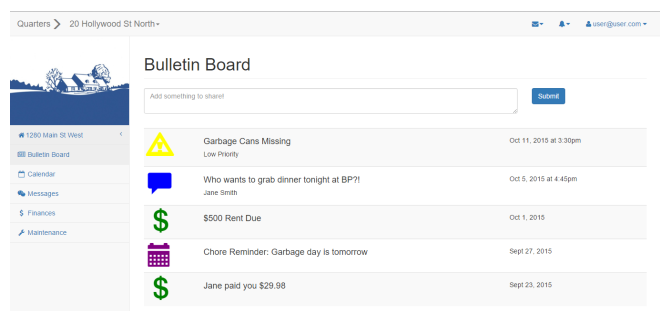
\includegraphics[width=\textwidth]{bulletin}
        \caption{Screen image of Bulletin Board page}
        \label{fig:bulletin}
    \end{figure}

    \subsubsection{Viewing the Bulletin Board}
    \begin{itemize}
        \item The bulletin board will be the first page loaded upon selecting a house
        \item Otherwise clicking on the bulletin board item in the sidebar will redirect you to the bulletin page
    \end{itemize}

    \subsubsection{Creating a post}
    \begin{enumerate}
        \item Click on the new post button, a modal will appear
        \item Fill out information in the modal window
        \item Files may be attached if necessary
        \item Click on create, the post will be created and added to the bulletin board
    \end{enumerate}

    \subsubsection{Replying to a post}
    \begin{enumerate}
        \item Click on view more replies
        \item Post will expand and display other replies
    \end{enumerate}

    \subsubsection{Deleting a post}
    \begin{enumerate}
        \item Post can only be deleted its the user's own post
        \item Lick on the ``Modify'' and a confirmation window will appear
        \item Clicking on yes will remove the post and close the window
    \end{enumerate}

    \subsubsection{Filtering post types}
    \begin{enumerate}
        \item Click on the types button on the top left, this will display a dropdown menu with different types
        \item Select the type the desired type
        \item Display will be updated with posts displayed from that specific type
    \end{enumerate}


    \subsection{Finance}
    To access the Finance page, click on "Finance" under the navigation bar. The Finance page displays a list of all "shared bills" to be split between tenants in the house. It keeps track of when the bills occurred, its participants, how much is owed by each person, and whether they've paid or not.

    \subsubsection{Add a bill}
    \begin{enumerate}
        \item To add a bill, click on the "+" button at the top of the Finance page. A pop-up modal will appear with the fields for user input.
        \item Select an event type for the bill(choose "other" if none of the predefined type applies)
        \item Fill out a description of the bill
        \item Pick the date the bill took place
        \item Choose the name of a payee of the bill
        \item Enter the amount that payee owes
        \item Click "Add"
        \item Repeat step 5-7 for other payees
        \item Click "Save" when all informations are filled out
    \end{enumerate}

    \subsubsection{Mark bill as "Paid"}
    Once a portion of the bill has been paid, the payee or the payer can mark that portion of the bill as "Paid"
    \begin{enumerate}
        \item Click on "Pay now" button beside the bill
    \end{enumerate}




    \subsection{Maintenance}
    To access the Maintenance page, click on "Maintenance" under the navigation bar. The Maintenance page displays a list of all the maintenance tickets created in the house in chronological order. It  allows a user to send maintenance requests to another user for them to address and resolve. Any user can send a request to any user in the same house. Each request has a priority level assigned to it to inform the receiver of the urgency of a response. Figure \ref{fig:maintenance} shows a screen image of the Maintenance page.

    \begin{figure}
        \centering
        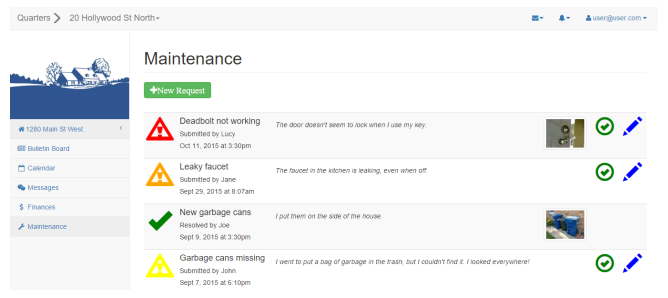
\includegraphics[width=\textwidth]{maintenance}
        \caption{Screen image of Maintenance page}
        \label{fig:maintenance}
    \end{figure}

    \subsubsection{Add a Ticket}
    \begin{enumerate}
        \item To add a ticket, click on the "New Request" button' at the top of the Maintenance page. A pop-up modal will appear with fields for user input.
        \item Fill out the fields. Note: All fields marked with an asterisk (*) must be filled.
        \item Click the "Submit" button at the bottom of the modal. The modal will close.
        \item The new request will display at the top of the Maintenance page above all of the other tickets.
    \end{enumerate}

    \subsubsection{Edit a Ticket}
    Only the creator of a ticket can edit the same ticket.
    \begin{enumerate}
        \item To edit a ticket, click on the blue pencil to the right of the relevant ticket. A pop-up modal will appear with editable fields.
        \item Edit the appropriate fields.
        \item Click on the "Submit" button at the bottom of the modal. The modal will close.
        \item The updated ticket will display in its original ordering.
    \end{enumerate}

    \subsubsection{Delete a Ticket}
    Only the creator of a ticket can delete the same ticket.
    \begin{enumerate}
        \item To delete a ticket, click on the red "X" to the right of the relevant ticket. A confirm modal will appear.
        \item Click "OK" to delete the ticket. The modal will close.
        \item The deleted ticket will no longer be displayed.
    \end{enumerate}

    \subsubsection{Resolve a Ticket}
    Only the receiver of a ticket can resolve the same ticket.
    \begin{enumerate}
        \item To resolve a ticket, click on the green checkmark to the right of the relevant ticket. A confirm modal will appear.
        \item Click "OK". The modal will close.
        \item The resolved ticket will display at the top of the Maintenance page above all of the other tickets. A green checkmark will replace the priority level symbol that was originally displayed on the left of the ticket.
    \end{enumerate}


    \subsection{Calendar}
    To access the Calendar page, click on "Calendar" under the navigation bar. The Calendar page displays a calendar showing all events created by members of the same house. Any user can add an event to the house's calendar. Figure \ref{fig:calendar} shows a screen image of the Calendar page.

    \begin{figure}
        \centering
        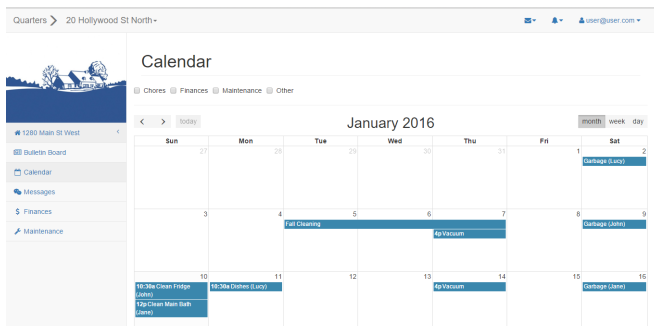
\includegraphics[width=\textwidth]{calendar}
        \caption{Screen image of Calendar page}
        \label{fig:calendar}
    \end{figure}

    \subsubsection{Change Calendar View}
    \begin{enumerate}
        \item The default calendar view is monthly. To change the calendar view, above the calendar, to the right, click the "Month" or "Week" or "Day" button. The calendar view will change.
    \end{enumerate}

    \subsubsection{Move Forward or Backward}
    \begin{enumerate}
        \item To move the calendar forward to the next month/week/day,  above the calendar, to the left, click the "$>$" button.
        \item To move the calendar backward to the previous month/week/day,  above the calendar, to the left, click the "$<$" button.
    \end{enumerate}

    \subsubsection{Add an Event}
    To add an event to the calendar, there are two methods: \\
    Method 1:
    \begin{enumerate}
        \item Navigate to the desired day (and time if in week or day view).
        \item Click on the desired day (and time if in week or day view). A pop-up modal will appear with fields for user input.
        \item Fill out the fields. Note: All fields marked with an asterisk (*) must be filled.
        \item Click the "Submit" button at the bottom of the modal. The modal will close.
        \item The new event will display on the calendar.
    \end{enumerate}
    Method 2:
    \begin{enumerate}
        \item Click on the "New Event" button at the top of the Calendar page. A pop-up modal will appear with fields for user input.
        \item Fill out the fields. Note: All fields marked with an asterisk (*) must be filled.
        \item Click the "Submit" button at the bottom of the modal. The modal will close.
        \item The new event will display on the calendar.
    \end{enumerate}

    \subsubsection{Edit an Event}
    Only the creator of an event can edit the same event.
    \begin{enumerate}
        \item To edit an event, navigate to the desired event on the calendar.
        \item Click on the desired event. A pop-up modal will appear with editable fields.
        \item Edit the appropriate fields.
        \item Click on the "Submit" button at the bottom of the modal. The modal will close.
        \item The updated event will display on the calendar.
    \end{enumerate}

    \subsubsection{Delete an Event}
    Only the creator of an event can delete the same event.
    \begin{enumerate}
        \item To delete an event, navigate to the desired event on the calendar.
        \item Click on the desired event. A pop-up modal will appear.
        \item Click on the "Delete" button beside the "Submit" button at the bottom of the modal.  A confirm modal will appear.
        \item Click "OK" to delete the event. The modals will close.
        \item The deleted event will no longer be displayed on the calendar.
    \end{enumerate}

    \subsection{Notifications}
    Various alerts will be sent to the user when requested. They can be viewed in the notifications dropdown as well as the notifications page.
    These notifications include updates and changes in a bulletin post, tagged in finance, ticking or bulletin post, upcoming events in calendar etc.
    \subsubsection{Viewing Notifications}
    \begin{enumerate}
        \item Clicking on the bell icon on the navbar will dropdown
        \item Latest notifications can be viewed here
        \item Further alerts can be found by click on the last item in the drop down "View all notifications";
    \end{enumerate}
    \subsubsection{Accessing post related to notification}
    \begin{enumerate}
        \item Open the notification dropdown or in the overall notification view
        \item clicking on an item will redirect you to post's page
    \end{enumerate}


    %%%%%%%%%%%%%%%%%%%%%%%%%%%%%% Troubleshooting
    \section{Troubleshooting}

    %%%%%%%%%%%%%%%%%%%%%%%%%%%%%% Frequently Asked Questions
    \section{Frequently Asked Questions}

    %%%%%%%%%%%%%%%%%%%%%%%%%%%%%% Safety and Precautions

\end{document}
